\section*{Des îles et des espèces}\label{des-uxeeles-et-des-espuxe8ces}
\addcontentsline{toc}{section}{Des îles et des espèces}

\subsection*{En suivant Wallace,}\label{en-suivant-wallace}
\addcontentsline{toc}{subsection}{En suivant Wallace,}

Dans l'introduction de son livre ``Island Life'' paru en 1881, le
célèbre naturaliste Alfred Russel Wallace nous rapporte deux faits
étonnant qui justifient pleinement l'examen attentif de la répartition
géographique des espèces (Wallace, 1881). Premièrement, la biogéorphe
montre avec des exemples multiples que l'éloignemnet de deux régions du
monde n'est pas suffiant pour conclure quand à l'éloignement de leur
composition faunistique et floristique. Ainsi, comparer les groupes
d'oiseaux de l'île japonnaise d'Hokkaido avec ceux de l'Angleterre,
pourtant séparés par des miliers de kilomètres, révèle une proximité des
paysages ornithologiques bien supérieure à celle constatée entre les
îles indonesiennes de Bali et de Lombok distantes de quelques dizaines
de kilomètres seulement. Deuxièmement, en s'appuyant sur les différences
des faunes brésiliennes et africaines sous des latitudes similaires,
Wallace souligne la faiblesse du pouvoir prédictif des variables
climatiques pour décire les compositions fauniques. Par la mise en
évidence de ces deux éléments, Wallace souligne le besoin de croiser les
informations des distributions à la lumière d'une analyse taxonomique.
Dans le cadre de la théorie de l'évolution\footnote{Wallace a publié en
  1858 un article \emph{On the Tendency of Varieties to Depart
  Indefinitely From the Original Type} qui témoigne très clairement que
  ses idées sur les varitions temporelles des espèces étaient très
  proche de celle de Charles Robert Darwin a qui il avait d'ailleurs
  envoyé le manuscipt (Wallace, 1858).}, encore toute jeune en 1881,
cette analyse taxonomique est en fait une analyse historique. Wallace
affirme ainsi que la compréhension d'un problème spatial, celui des
aires de répartition de groupes d'espèces proches, n'est possible que
par une compréhension temporelle, celle de l'histoire des espèces, cette
idée est clairemnt énoncée dans la même introduciton :

\begin{quote}
« Many years study of this class of subjects has convinced me that there
is no short abd easy method of dealing with them; because they are, in
their very nature, the visible outcome and residual product of the whole
past history of the earth. »
\end{quote}

Tout au long de son livre, Wallace démontre que la connaissance à
l'échelle mondiale de la distribution des êtres vivants à travers le
monde permet de relier les différentes îles aux grands ensembles
régionnaux biologiques (que nous appelons aujourd'hui écozones) et que
ces groupes sont aussi relié par des liens historiques dont la taxonomie
révèle les traces. Ce travail de charactérisation d'ensemble
géographique conduit Wallace, dans un article de 1860 (Wallace, 1860), à
tracer la ligne séparant l'écozone indomalaise de l'écozone australienne
(qui sépare notamment Bali et Lomonk citées plus haut) qui porte encore
aujourd'hui son nom. L'éclaircissement de la géographie par l'histoire
est saississant et les exemples de Wallace sont autant de poids données
à la théorie de l'évolution. Le discours de Wallac porte sur des
processus à des échelles spataile et temporelles très grandes,\footnote{L'âge
  de la terre est très débattu à l'époque bien que de nombreux s'accore
  que les 6000 ans biblique sont insuffisant, Wallace avance,
  audacieusemnt, l'age de 500 milians d'année.} et bien que
l'éclaircissement substantiel des répartitions géogrpahiques des êtres
vivants par l'évolution, cette expliqcation se double d'un obstacle
épistémologique important : si l'explication ultime de la présence d'une
espèce en un point donné est le produit d'une série de contingences
historiques, sur quoi bâtir une théorie de la biogéographie? Ce n'est
qu'au XX\^{}ème siècle que des réponses convaincaites émergeront avec a
fructuseuse rencontre du mathématicien et biologiste Robert Helmer
MacArthur et du myrmécologue Edward Osborne Wilson.\footnote{Cet actuel
  professeur émérite à l'université d'Harvard est reconnu pour ces
  apport en biologie et en sociologue, il est l'auteur de 32 livres mais
  c'est pour son immense connaissance des fourmis que j'ai choisi
  l'adjectif de myrmécologue.}

\subsection{En suivant MacArthur et
Wilson}\label{en-suivant-macarthur-et-wilson}

La collaboration de ces deux jeunes biologistes a mené à la formulation
d'une théorie de la biogéographie insulaire publiée en 1967 sur laquelle
je reviendrai abondammnent tout au long de mon introduction (MacArthur
and Wilson, 1967) puisqu'elle est un des piliers de ma thèse. Leur
démarche a été de collecter un grand nombres de données sur différents
groupe d'espèces sur des îles dispersées un peu partout dans le monde et
pour essayer de mettre une cohérence à travers ces faits avec un cadre
théorique puissant. Comme indiqué au au dernier chapitre de leur livre
de 1967, ces auteurs souhaite voir la biogéographie entrer dans une
nouvelle phase :

\begin{quote}
« Biogeography has long remained in a natural history phase,
accumulating information about the distribution of species and higher
taxa and the taxonomic composition of biotas. Interpretative reasoning
has been largely directed to the solution of special problems connected
with the histories of individuals taxa and biotas. Without doubt this
descriptive activity will continue to be of fundamental importance to
the science, one of the most physically adventurous of all scientific
entreprises and, in the richness of the detail it unfolds, esthetically
pleasing. But biogeography is also in a position to enter an equally
interesting experimental and thereotical phase. »
\end{quote}

MacArthur et Wilson affirment que l'étude de la distribution des espèces
doit sortir du royaumes des contingences pour devenir un objet de
science au sens d'être manipulé aussi bien expérimentalement que par
l'abstraction mathématique. La validation expérimentale de la théorie a
été menée par Wilson et son étudiant au doctorat de l'époque, devenu
depuis le grand écologue Daniel Simberloff, avec une expérience de
défaunation de six petits îlots de mangrove dans la Baie de Floride
(Simberloff and Wilson, 1969). La travail d'abstraction mathématique a
été conduit par MacArthur dans le livre de 1967 et prolongé dans les
annexes de son livre de 1972 (MacArthur, 1972). Leurs efforts conjugués
ont donné le jour à une vision puissante de la biogéographie dans
laquelle la richesse spécifique d'une île donnée est le résultat de deux
porcessus oposés : un processus de colonisation qui augmente le nombre
d'espèce sur l'île et un porcessus d'extinction qui le diminue. En
reliant ces processus aux propriétés physiques de l'île (aire et
isolation) et en interprétant la richesse spécifique des îles en terme
d'équilibre entre ces deux processus, les auteurs parviennent à
expliquer de manière convaincante les relations observées entre richesse
spécifique, taille de l'île et isolement (je reviens amplement sur cette
théorie dans le troisième temps de cette introduction).

Le paradigme données par les auteurs est un lègue qui a eu un impact
considérable sur les développemnt théorique en écologie (Warren et al.,
2015). Au coeur de la réussite du modèle, il y a la vonlonté de mettre
l'espèce au coeur de la biogéographie de ne pas simplemnt parler de
grands ensembles régionaux et d'em discuter l'histoire nais aussi de
coprendre les mécanismes biologiques plus fins qui sont le moteur
essentiel de la variation dans la distribution des espèces. Tout
l'intérêt de leur \emph{biogéographie de l'espèce} (terme donné à
l'avant-dernière phrase de leur livre de 1967) est dans l'affirmation
qu'il faut repgarder les contraintes conjointe de l'évolution (qui met
un certain nombre de groupes taxonomiques en présence) et du context
écologique qui régit les conditions d'extinction. Cette intrication de
l'écologie et de l'évolution est bien inscript dans la pensée de
MacArthur et Wilson même si la puissance de leur vision réside dans le
fait de les occulter en partie.

Près de 50 and après la parution de leur livre, une des clef en biologie
semble être la compréhesion des retro actions l'écologie et de
l'évoluton dans les varitions spatiale et temporelles de la
biodiversité. On peut reprendre les trois aphorismes cités par Schoener
(2011a) :

\begin{quote}
« Nothing in biology makes sense except in the light of evolution. »
(Dobzhansky, 1964)
\end{quote}

\begin{quote}
« This was supplanted half a century later by (2): Nothing in
evolutionary biology makes sense except in the light of ecology. »
(Grant and Grant, 2008)
\end{quote}

\begin{quote}
« Nothing in evolution or ecology makes sense except in the light of the
other. » (Pelltier, 2009)
\end{quote}

Au sein de la communauté, l'idée qu'il est difficle d'isoler les deux
discipline et cela indépendamment de l'échelle cnsidérée semble gagner
du terrain. Un parrallèle avec les sciences humaines me semble possible
l'écologie serait à la biologie ce que la géographie est aux sciences
humaines et aussi que l'évolution serait à la biologie ce que l'histoire
est aux sciences humaines. Nous pouvons bien sur étudier l'une sans
l'autre, mais le dialogue entre les deux disciplines est indispensable
sinon elles avancent en faisant des hypothèses fortes sur l'autre et qui
finiront éventuellement par nuire à la compréhension. Aisin supposé que
les ressort de la varation sont puremnt des mécanimes écologique alros
que dans certains système la variation allélique peut affecter
rapidement et formtement la démogrpahie est problématqie (Pelletier et
al., 2007). Néanmoins chaque discipline a des connaissance à apporter
pour nourir ce dialogue et la Biogéogrpahie est le champ qui tente de
conprendre l'information refermée dans les distributions d'espèces.

\subsection*{Quelles informations renferment les distributions
d'espèces?}\label{quelles-informations-renferment-les-distributions-despuxe8ces}
\addcontentsline{toc}{subsection}{Quelles informations renferment les
distributions d'espèces?}

Cette question est non seulement une invitation à découvrir les raisons
de la présence de tel ou tel organisme en un lieu donné du globe, mais
elle suggère ausi que certaines informations ne sont pas obtenue par
l'analyse de répartion géographique des espèces. Les grands auteurs
mentionnés dans les paragraphes précédents y ont apporté des éléments de
réponse essentiels : Wallace a montré que la distribution reflètait en
partie les liens de parenté entre les esèces, quant à MacArthur et
Wilson, ils ont suggérés que ces distributions étaient le résultats de
processus écologiques dynamiques. Examiner les aires de répartition,
relever les variations spatiales et temporelles, mais aussi détailler la
géométrie exacte au regad de variables abiotique ou à la lumière de la
géométrie d'autres espèces est une clief pour apprécier les mécanismes
sous-jacents.

Dans son ouvrage de 1972, MacArthur se livre à un examen approfondi du
sujet en examinant des aires de répartition au regard des variables
climatiques mais aussi les variations teporelles ou encore les relations
qu'il existe entre les distributions d'espèce en compétition. Il propose
un cadre mathématique pour comprendre l'impact de la prédation et de la
compétition sur lequel repose un prinicpe de ségrégation spatiale
d'espèce en compétition : deux compétiteurs ne peuvent pas co-occurer
(être trouver au même endroit) sauf éventuellement sur zone très
restreinte de leur distribution (MacArthur, 1972). Toujours dans ce même
ouvrage, MacArthur évoque la distribution en damier
(\emph{checkerboard}) que peuvent générer des espèces en compétition. Ce
type de distribution sera approfondie et quantifiée par Jared Diamond
(Diamond, 1975) dont les travaux déclencheront un débat important sur la
determination de modèle null de co-occurrence (Connor and Simberloff,
1979).

L'analyse des distributions d'espèce est riche quand l'anaylse a de
multiple approche. Bien entendu dans un premier temps, l'examen sur de
multiple aires de répartition est un premier pas pour y déceler des
phénomènes répétés nécessaires à l'élaboration des th.éories (MacArthur,
1972). C'est aussi dans l'examen des variations spatiales et temporelles
que les informations abondent car si ces variations sont par exemple
reflétées dans els changelmnts climatiques, cela justifie l'espoir de
comprendre l'évolution des distributions d'espèces dans un context de
chanmgement climatique. De plus, l'examen d'une distribution est aussi à
faire par comparaison avec d'autre espèces notamment les espèces en
interaction pour voir si la biologie laisse ces empreintes dans la
géométrie de ces aires de répartition. C'est ainsi que dans ma thèse, je
propose de regarder l'intersection des aires d'un ensemble de proies
pour comprendre ce que la co-occurrrence peut nous apprendre.

\subsection*{Enjeux de la connaisssance de la répartition géographique
des
espèces}\label{enjeux-de-la-connaisssance-de-la-ruxe9partition-guxe9ographique-des-espuxe8ces}
\addcontentsline{toc}{subsection}{Enjeux de la connaisssance de la
répartition géographique des espèces}

Les enjeux fondamentaux ont été évoqués plus haut : les observations et
la compréhension des causes profondes de la géométrie et la dynamique
des aires de répartitions des espèces ont déjà amené à des découvertes
majeures en écologie et en évolution. La phase d'expérience et de
Théorie décite par MacArthur et Wilson se poursuit et l'espoint se
tourne vers la possibilité d'obtenir des prédictions fiabkes sur les
aires de répartitions futures d'une espèce données. Ce problème est
d'autant plus pesant dans la litérature en biogéograhique dans le
contexte actuel des changements globaux. En biogéogrpahie, les
changements climatiques ont canalisés l'attention et les chercheurs
constatent l'ampleur à laquelle la biodiversité mondiale est affectée
par ces derniers (Koh, 2004, Bellard et al. (2012)). Le volonté
d'anticiper où seront les espèces demain a également engendré un effort
de développemnet d'outils statistiques essentiellement centrés sur la
correlation entre les variables abiotiques et occurrence des espèces
(Elith et al., 2006).

En choississant de parler de telle ou telle espèce, nous glissons
rapidement à des enjeux sociaux et économiques évidents. Ainsi, pour un
pays comme la France, comprendre les impacts des changements climatiques
sur la productions du vin est un enjeu central, prédiction de
contractions des aires de production favorables dans les grandes régions
viticoles (Hannah et al., 2013), on peut aisément deviner ou seront les
grands vignobles de demain à de multiple conséquences économiques sur
les cours des vins, les millésimes, le prix de ces terres agricole. Pour
aborder un exemple québécois, posons la question suivant : où seront les
érablières de demain? La réponse à cette question réside dans la
détermination de la répartiton future des aires favorable à la
croissance de l'érable à sucre (\emph{Acer saccharum}) mais aussi de
leur possibilité de migrer efficacemnet pour s'y installer. Bien que les
prédictions des modèles d'évolution de la composition des forêts borel
au nord du Québec fassent des prédictions sur la Baie d'ungava il semble
que le taux de migration empêche d'atteindred ces terres éloignés à
moins d'envisager des migrations assistée. Je finirais par un troisième
exemple celui souvent mis en évicende de la perte des pollinisteurs et
notamment des abeilles. Pas moins de quatres grandes classes de facteurs
d'origine anthropique les mettent en dangerr : , les changements
climatiques, le chagement de l'utilisation des terres\footnote{Changements
  accompagnés, entre autres, de l'utilisaion parfois massive de
  pesticide de la famille des néonicotinoïdes affaiblissant les
  colonies.}, l'apparition de nouveaux pathogenès (dont l'accarien
parasite \emph{Varroa destructoa} vecteur de nombreux virus) (Vanbergen,
2013). Le défi actuel est donc de prédire la distribution future en
intégrant ces mutiples aspects et donc la distribution d'espèce en
interaction qui ne peuvent donc êtres traitées séparément.

Actuellement, les outils de prédictions des aires de répartition future
reposent essentiellement sur les scénarios de changments climatiques
(RCP). La démarche est cohérente, la connaissance basée sur les
corrélation de variable climatique dont les climatologues sont en mesure
de fournir des gammes d'estimation relativement fiables qui sont une
base de reflexion importante sur les zones favorables à ;a croissance
des différentes espèces. Mais les porblénatiques d'invasion d'espèces
nous rappellemnt que nous sommes souvemt en mesure de comprendre le
potentiel invasof seulemnet a posyteriori. Ces porblèmes de qualit. de
distribution sont le reflet de lacune théorique qui amène les chercheurs
à se positionnier en faveurs d'un renouvellemnt théorique avec l'objecif
de la création d'une biogéographie intégrative capable de préiction
fiables (Lomolino, 2000, Beck et al. (2012), Thuiller et al. (2013)).
Biensur ces appels soulèvent des défis techniques et théoriques
importants dont on ne peut qu'espèrer qu'il soit relevé au plus vite en
dépit de l'urgence.

\subsection*{Travail théorique et
modélisation}\label{travail-thuxe9orique-et-moduxe9lisation}
\addcontentsline{toc}{subsection}{Travail théorique et modélisation}

Avant d'énumérer, avec des exemples concrets, l'ensemble des forces qui
régissent la répartition géogrpahique d'une espèce, je précise dans
cette partir l'importance du travail de théorie et de modélisation qui
tient une place importante dans ma thèse.

\subsubsection*{Rassembler et intégrer des
faits}\label{rassembler-et-intuxe9grer-des-faits}
\addcontentsline{toc}{subsubsection}{Rassembler et intégrer des faits}

Le travail de théorie est avant tout la mise en cohésion d'un certain
nombre de faits. Dans leur théorie de la Biogéograohie des îles, les
auteurs parviennet à montrer que les relations en terme de richesse
spécifique s'exlique bien, dans les données qu'ils possèdent, par la
connaissance combiner de l'isolement des îles et de leur taille. Il y a
également deux principes principes qui encadrent la construction d'une
théorie scientifique : elle demeur valide lorsqu'elle n'est pas prouvé
fausse et qu'une alternative ne la supplante pas, elle doit être
parcimonieuse, ne pas invoquer de multiple processus sans raison, c'est
ce que l'on appelle parfois le Rasoir d'Ockham. C'est qu'une boutade,
dont je ne suis pas capable de rapporter son auteur, indique que les
physiciens expliquent 95\% de l'univers avec 5 règle alors que les
économistes expliquent 5\% des phénomènes qu'ils étudient avec 95
règles.\footnote{On peut trouver une variante énonçant que les
  économistes ont pédit 12 des trois dernières crises économiques. Je
  pense qu'au point de vue de la qualité des prédictions en
  biogéogrpahie, nous nous apparentons plus aux economistes qu'aux
  physiciens.} Le problème n'est pas tant de dénigrer une discipline
mais de constater la puissance prédictive d'une théorie problèmes que
posent actuellement la prédictions en économie. C'est peut-être le
reflet d'une maturité pour la physique il n'en demeure pas moins que des
défis majeur et de grands questionnement la traverse. La théorie est une
construction mentale qui permet de donner un cadre de penser et ce
dernier peut être explorer à travers des modèles.

\subsubsection*{Des modèles pour explorer la
théorie}\label{des-moduxe8les-pour-explorer-la-thuxe9orie}
\addcontentsline{toc}{subsubsection}{Des modèles pour explorer la
théorie}

Le terme de modèle signifit simplement que l'objet en question à des
propriétés bien connu. Ainsi un organisme modèle est un organisme sur
lequel souvent facile à elever et maniupluler sur lequel beaucoup de
connaissance nt été établis et qui sert d'unité empirique à travers un
ouo plusierus laboratoires. Quand on travail sur des modèles statisique,
on connait exactement le type de correlation que l'on entreprend. De
même pour un travail de modellisation mathématique, la description du
modèle est contenu dans une série d'équations. Un modèle est souvent
perçu comme une simplification de la réalité, en effet, comment
prétendre que les mécanismes biologiques décelés chez \emph{Arabidopsis
Thaliana}\footnote{Il s'agit de la plante modèle par excellence le
  génome le permier à être séquencé chez les plantes (Arabidopsis Genome
  Initiative, 2000).} sont les mênes pour l'ensemble des plantes à
fleurs? Pour combien de système proie-prédateur le modèle de
Lotka-Volterra est-il pertinent?

Les limites des modèles doivent être reconnues mais il ne faut pas nier
l'apport de ces derniers. Ainsi les modèles sont autant de chance pour
explorer une ou plusiers prédiction d'une théorie. Le choix du modèle
est laissé au chercheur, comme le rappelle Kevin McCann dans la préface
de son livre \emph{Food Webs} (McCann, 2011):

\begin{quote}
« It just so happens that some people find it easier to think about
things in terms of x's and y's, and other in terms rabbits of and lynx.
»
\end{quote}

En d'autres termes, certains on plus de faciliter pour penser en termes
mathématiques et d'autres en termes expirimentaux. Je suis plutôt dans
la première catégorie de personne, je pense que les mathématiques sont
un cadre de penser très puissant comme l'indique le grand écologue
Robert McCredie May (May, 2004):

\begin{quote}
the virtue of mathematics in such a context is that it forces clarity
and precision upon the conjecture, thus enabling meaningful comparison
between the consequences of basics assumptions and the empirical facts.
Here mathematics is seen in its quintesence : no more, but no less, than
a way to think clealy.''(p.~791, (May, 2004))
\end{quote}

Dans ma thèse j'ai essayé d'utilisé les mathématiques pour développer
des modèles qui sont surtout parti de reflexion collective autour du
rôle que pouvaient jouer les interactions dans les distrbution d'espèce.
Cette reflexion m'a parmis d'établir des prédictions dont certaines
semblent être vérifiées.

\subsubsection*{Nouvelles prédictions}\label{nouvelles-pruxe9dictions}
\addcontentsline{toc}{subsubsection}{Nouvelles prédictions}

Après l'établissent d'un théorie suportée par un certain nombre de fait,
le cadre conceptuel qu'elle propose étant travailler autour de travaux
expérimentaux et de modélisations, de nouvelles prédictions émergent. La
vérificaton des prédictions autour de nouvelles expérience et si elles
sont vérfiée la théorie en sera renforcer. Ces dernières années, la
physique nous a donnée des exemples très importants ces dernières années
de vérification de théorie énoncée bien avant que les outils permettant
de mettre au point leur vérification existent : la détection, validée en
2012, du Boson de Higgs dont l'éxistence a été prédite énoncée en
1964\footnote{Pour plus de détail au bulletin du CERN
  {[}http://cds.cern.ch/journal/CERNBulletin/2012/28/News\%20Articles/1459456?ln=fr{]}{[}http://cds.cern.ch/journal/CERNBulletin/2012/28/News\%20Articles/1459456?ln=fr{]}}
et la détection des ondes gravitationelles cette année soit 100 ans
après qu'Einstein en ait prédit l'existence (Waldrop, 2016). Dans le
cadre de la biogéographie, la validation d'une théorie puissant em
Biogéogrpahie pourrait être possible si les aires de répartition
futurtee sont préditcte correctment et si les pertes d'espèces, les
conséquence de l'introduction de telles ou telle espèces sont validées.
Pour y parvenir, cela demande d'être en mesure de connaître l'ensemble
des nécanimses qui interviennet dans le tracé des aires de répartiton,
comment ces pricessus interagissent et quels sont leurs imprtances
relatives.

\section*{Répartition géographiques des espèces, les forces en
présence}\label{ruxe9partition-guxe9ographiques-des-espuxe8ces-les-forces-en-pruxe9sence}
\addcontentsline{toc}{section}{Répartition géographiques des espèces,
les forces en présence}

\subsection*{Biogéographie
historique}\label{bioguxe9ographie-historique}
\addcontentsline{toc}{subsection}{Biogéographie historique}

Il s'agit du récit des variations temporelles à larges des échelles
temporelles. C'est dans l'étude de la proximité des taxons mais aussi
des fossiles éventuels que l'on déchifre comment certains groupes ont
colonisés tels ou tels lieu. La théorie de la dérive des continents
établie par Alfred Lothar Wegener, notamment basée sur la similarité de
fossiles trouvés sur des continents très èloignés, implique que des
groupes éventuellement proche il y a des milions d'année ont été séparée
et on donnaée maissane à des lignées différentes. Aujourd'hui nous
sommes capables de retracer ces liens de parenté à l'aide de phylogénies
moléculaires sont des outils très efficace pour comprendre depuiis quand
les différents taxons ont été séparée. Par la compairaison des génômes
motochindiriaux, il a été montré récemment que les lémuriens (primates
malgaches) ont été séparées de toute autre lignée de primates il y a 60
milions d'année environs (Finstermeier et al., 2013). Une autre partie
du travail devant ces faits est de comprendre quels ont été les
mécanismes qui ont conduit à l'isolation de ce groupe de singes à
Madagscar et à la construction des communautés que nous observons
actuellement (Razafindratsima et al., 2013).

Les processus de grande amplitude temporelle sont cependant dominés par
le poids historique et prédire un phénomène tel que l'extinction des
dinosaurs n'est chose aisée qu'une fois qu'il s'est déroulé. Cela dit,
en regardant des évènemnets plus récents, certains mécanimes puis être
mis en jeu. Aisin, l'étude de la diversification des bouziers entrepris
par Joachim Hortal et collègues (Hortal et al., 2011) montre que la
dernière glacition qui a cntraint le range de ces espèces sesibles au
froid, a laissé des empreintent encore visible dans la diversité de ce
groupe : la limite de la thermocline 0°C durant le dernier maximum
glacier ( il ya 21000 ans environs) sépare les zones de fortes diversié
en bouzier. De plus, ils montrent que la diversité phylogénique des
espèces plus au nord, c'est-à-dire plus tolérante au froid, est un
sous-ensemble phylogénétique très restrient, c'est à dire que peu de
branches de ces bouziers sont à l'originie des colonisations nordique.
Ainsi après uen conrtaction des ranges, il y a une empreinte sur la
diversification des espèces et ceux malgrés leur capacité de dispersion
(Hortal et al., 2011).

\subsection*{Capactés de dispersion et structure du
payasage}\label{capactuxe9s-de-dispersion-et-structure-du-payasage}
\addcontentsline{toc}{subsection}{Capactés de dispersion et structure du
payasage}

La remonté nordique des bouziers depuis le dernier maximum glacier
signalé au pargraphe précédent est sans doute lié à des évènemnets de
dispersion à l'échelle individuel. Le mouvement des individus les
conduit au fil des générations à se disperser et si le milieu est
favorable à y perdurer. Ces mouvements individules ont des
répercusssions à l'échelles de l'espèce. Il s'agit là d'un moteur
essentiel de la répartition des espèces : le lien à l'espace. Même les
espèces sessile omt des capacit.s de dispersion par la production de
semence disséminé par toute sorte de mécanisme. La diffusion des
organimes est inévitable comme une forme d'entropie, cette comparaison
est intéressante car elle montre que des mouvements stochaistqies
conduisent à une forme de dispersion assez prévisible.

Le cadre de diffusion est néanmoins cintraint par la structure du
paysage. On peut parler de conraintes physique : vallé encastré autour
de montanges difficiles à passée, une rivière, des vents ou des courants
dominants qui dirigent les mouvemnets de dispersion. Mais aussi le
climat dans arrivés, les différentes espèces en présene. Aussi
contraintes les échemnges entre population et modelée les flux de gènes
qui traversent les popylatons (Metapopultion ont montré que différents
porblème oour abirder (Leibold et al., 2004)).

Mais des conséquence prévisibles expérice de d.foliation. Après avoir
défolié

\subsection*{Environnement abiotique et distribution des
espèces}\label{environnement-abiotique-et-distribution-des-espuxe8ces}
\addcontentsline{toc}{subsection}{Environnement abiotique et
distribution des espèces}

Dans le chapitre 6 de son livre de 1972 \emph{Geographical Ecology}
MacArthur (1972) présente l'importance des contraintes climatiques à
travers l'exemple de l'aire de répartition du cactus Saguaro
(\emph{Cereus giganteus} dans le livre mais aujourd'hui \emph{Carnegiea
gigantea},
http://www.itis.gov/servlet/SingleRpt/SingleRpt?search\_topic=TSN\&search\_value=506151).
Ce résident du désert de Sonora est sensible au gel et ne peut resister
à une exposition de quelques dizaines d'heures au gel. Cette contrainte
physiologique explique bien les limites nord et est de sa répartition.
Pour la limite sud (la limite à l'ouest étant l'océan pacifique), il
semble que l'abondance des pluie hivernale ne lui soit pas favorable.
Ces résulats semble confirmer ar des travaux récents qui prédise un
changement et ajoutent que le l'augnetation du feu pourrait avoir des
conséquences négatives sur cette expansion (Springer et al., 2015).
Cette démarche de recherche active des limites climatiques recoupée aux
limites phuysiologiques est la détermination de la niche fundamnetal.
Cette approche a été poussé à son paroxysme dans l'article de Kearney et
Porter sur le petit gecko australien nocturne \emph{Heteronotia binoei}
(Kearney and Porter, 2004). Ils ont montrés qu'en combinant des mesures
physiologiques (dont le taux métaboliques au repos, le température
cumulées nécessaire au bon développement des oeufs et des mesures de
températures charactéristiques) avec des données climatiques, les
rpobbailités d'observations et les obsevatuons corrélaient et que cela
fondait la démarche prédictive de s'apuyer sur les scénarios de
changement climatiques pour aller essayer de comprender les réaprtitions
futures.

Cette approche s'apparentent à la recherche de facteurs limitants qui
sont le reflets de contrinate physiologiques. On peut encore cité
l'exemple fourni par Engelbrecht et al. (2007) qui ont montrés qu'au
niveau du Panama la distribution local et régionale de 48 espèces
d'arbres étaint bien expliqué par la sensibilité à la sécheresse, donc à
une variation dans la disponibilité d'une ressource. Ces corrélations
convaincantes fondent les modèles de distributions d'espéces (SDM
enréférence au terme anglais utilisé souvent dans le reste de la thèse)
qui cherche à faire correspondre les variables climatiques aux données
de co-occurrence (Elith et al., 2006, Elith and Leathwick (2009)). Le
succès récents de ces apporches a l'abondance des données climatiques
comme cellles porposées librement par WorldClim (données disponible en
ligne \url{http://worldclim.org}, Hijmans et al. (2005)) et la relative
faciliter d'abtonr des donn.es de co-occurrence qui tentent à être
égalment disponble en ligne comme le portail de données sur la
biodiversité à l'échelle mondiale GBIF (Global Biodiversity Information
Facility, \url{http://www.gbif.org}) malgré des biais lié à des efforts
différents dans les différentes régions du globe (Beck et al., 2014). Le
succès repose sur les besooin prédictif dans un contexte de changement
climatique qui conduisent à un effort de recherche important dans le
domaine \cite{Thomas2004,Thuiller2011}.

La niche fundamnetale est une contrainte de premier plan dircetemnt lié
aux relation des un ancrage important de la biogéographie. La théorie
doit non seulement permettre de comprendre mais aussi les articluations
avec les autres composante de la biogéographie que je détaille
ci-dessous. Importance théorique

\subsection*{Réseaux d'interactions : interdépendance des
espèces}\label{ruxe9seaux-dinteractions-interduxe9pendance-des-espuxe8ces}
\addcontentsline{toc}{subsection}{Réseaux d'interactions :
interdépendance des espèces}

Dans le même chapitre 6 de \emph{Geographical Ecology} MacArthur parle
clairement de la contrainte biotique notamment du rôle que peu avoir la
compétition pour comprendre la distribution des espèces. la prédation et
la compétition ont été très vote envisagée Il reprend l'exemple donnée
par Brown en 1971 de l'exclusion compétitive de deux espèces de de
tamias, \emph{Eutamias dorsalis} et \emph{E. umbrinus}, dans les forêts
d'altitude (au dess-su des déserts) de pins et de junipers
(\emph{pinyon-juniper woodland} woodland) du Sud outes des Etats-Unis.
L'article de Brown montre bien comment une différence comportementale
peu engendré une séparation des distirubution locales. Ainsi,
l'aggressivité de \emph{Eutamias dorsalis} lui est favorable dans les
forêts clersemés où son compétiteur doit dépensé beacoup d'énergie pour
se réfuugié dand un arbre de basse altidue alors que l'abondance des
arbres le rend inefficace, le compétiteur plus facilemnent y échappe.
Ainsi la segregation locale des deux espèces reflète bien une
interaction biotique et donc l'information contenu dans la distrbution
est aussi de nature très précise : competiton pour ressources et
comprtanemnt.

Au-delà de la competition, l'écologie des réseaux actuelle nous montre à
quel point il est difficile de concevoir les espèces comme
indépendantes, elles sont reliés par des relations de très diverses
natures. Les relations trophiques sont les plus évidentes, mais il
existe aussi une myriade d'interaction non trophiques qui affectent
aussi utlimement la démographie des espèces (voir Kéfi et al. (2012)
pour une relexion autour et une classification de ces interactions) et
il existe actuellemnt aucun argument solide justifiant la primauté d'un
tyoe d'nteraction sur les autres. Récemment, les interactions trophiques
et non-trophiques ont été exhaustivement analysées pour 104 espèces des
écosystèmes interdidaux rocheux de la partie centrale de la côte
chilienne révélant ainsi que les interactions non-trophiques y étaient
globalemnent plus abondantes et concentrées sur les bas niveau trophques
(Kéfi et al., 2015). La compréhension fine des lines qui existent entre
les êtres vivants est un ressort essentiel pour obtenir des théories
puissantes sur la dynamique des populations à placer au coeur de la
biogéograohie comme le mentionnait MacArthur et Wilson au dernier
paragraphe de leur Théorie de la Biogeographi insulaire par ces mots :

\begin{quote}
\guillemotleft In short, biogrography apperas to us ti hace develope to
the extent taht it cam be reformulated in terms of the first pricnciples
of population ecology and genetics. \guillemotright
\end{quote}

Le débat majeur autour de la relation entre la diversité et la stabilité
des écosystèmes au regard de la structure des réseaux (May, 1973,
Allesina and Tang (2012).) doivent être aussi regardé en terme de
conséquence sur le changement de réoartition des espèces. Le débat c'est
construit autour d'argymemnt mathématqieu qui ont considérablement
enrichit l'écologue (McCann, 2000) La représentation en réseau de ces
interactions est un outil puissant pour synthétiser la complexité des
écosystèmes ({\textbf{???}}, Pascual and Dunne (2006)). Avce une seule
matrice Ils sont représentés par la matrice de communauté qui résume
l'effet démographique des espèces par pair. Cette matrice renferme des
informations précieuses telles que la connectance (mesure du nombre de
liens constatés rapporté au nombre de liens possibles), la topologie des
interactions entre espèces \cite{Sole2006} et les effets indirects
(Wootton, 1994, Montoya et al. (2009)).

Il y a cependant deux problémes majeurs - abndance des interactions - la
distribution de mais ce signal disparait si l'on considère une avec un
grain plus grossier (voir section échelle). et abondance des
interactions ne sont peut être pass distincable

\subsection*{Eco-evo dynamqieu}\label{eco-evo-dynamqieu}
\addcontentsline{toc}{subsection}{Eco-evo dynamqieu}

Retro action des processus évolutifs vers une synthèse Schoener (2011b)

Les processus évolutifs peuvent être favorisés par les changements
environnementaux mais également par les interactions entre espèces
\cite{Tingley2009}. Les étroites relations entre espèces peuvent
favoriser ou contraindre les réponses évolutifs, qui elles-mêmes peuvent
altérées ces interactions, il existe de fait des rétroactions
permanentes entre évolution et écologie \cite{Post2009}. Yoshida
\textit{et al.} 2003 montrent que la réponse des algues vertes
unicellulaires \textit{Chlorella vulgaris} aux rotifères
\textit{Brachionus calyciflorus} conduit à un changement dans la
fréquence et la phase des cycles de la dynamiques proie prédateur
\cite{Yoshida2003}. L'ensemble des trois éléments jusqu'ici évoqués
(environnement abiotique, interaction, évolution) peuvent également être
étroitement associé. Grant et Grant 2006 rapportent le cas de la
compétition entre trois espèces de pinsons (dits de Darwin) sur l'ile de
Daphne (Galapagos) qui engendre une modification de la taille de leurs
becs. Cette évolution liée à la compétition est elle même reliée à
l'environnement abiotique car, par l'abondance ou l'absence de
précipitations, il détermine la disponibilité des ressources et donc
l'intensité de la compétition \cite{Grant2006}. A travers cet exemple,
nous comprenons l'importance d'inclure l'ensemble des différents
processus pour construire un modèle intégratif en biogéographie. Un tel
modèle serait capable, par exemple, de renseigner les risques
d'exclusion compétitive dans l'exemple décrit par Grant et Grant.

vers une systhèse Schoener (2011b) =\textgreater{}~interaction de ces
processus.

La vie telle que nous la connaissons pérennise l'information accumulée
au cours du temps via à un support moléculaire, l'ADN. Cette molécule
peut 1- renfermer une plasticité phénotypique offrant aux espèces des
possibilités pour faire face aux stress environnementaux et 2- subir des
altérations, des mutations, dont le relative avantage apporté peut
assurer une survie accrue. Les espèces sont donc elles-mêmes porteuses
potentielles de réponses face aux changement actuels
\cite{Parmesan2006,Lavergne2010}. La plasticité phénotypique permet une
réaction rapide des espèces à des changements environnementaux soudains.
Tingley \textit{et al.} 2009 ont ainsi montré que sur 53 espèces
d'oiseaux étudiés dans la Sierra Nevada, 48 ont colonisé de nouveaux
sites où les conditions de température et de précipitations leur étaient
plus favorables \cite{Tingley2009}. Les mutations sont quant à elles des
évènements relativement rares qui interviennent potentiellement à chaque
génération, leur fréquence est donc dépendante, en premier lieu du temps
de génération mais aussi de la tolérance des systèmes de réplication du
matériel génétique. Pour des espèces aux temps de génération court, les
processus micro-évolutifs peuvent donc être déterminants. Ainsi, Balanyá
\textit{et al.} 2009 ont montré des changements notables dans le
génotype de \textit{Drosophila subobscura} en 24 années avec des
génotypes de basses latitudes plus répandus en réponses au changements
climatiques.

Il est capital de ne pas oublier les processus évolutifs dans un modèle
de biogéographie afin d'envisager correctement la biodiversité de demain
\cite{Sexton2009,Lavergne2010}. La nature des processus à prendre en
compte est dépendante de l'échelle de temps considérée. Ainsi, si l'on
souhaite retracer l'histoire évolutive d'une région, les aspects
adaptatifs relevant de la micro-évolution sont moins pertinents que les
processus évolutifs de longue portée modifiant profondément les espèces.
Il faut, à ce propos, rappeler que l'évolution peut conduire à un
enrichissement du pool d'espèce d'une région donnée
\cite{Rosindell2011,MacArthur1967}. Les mutations accumulées dans une
population isolée géographiquement peuvent conduire à une
incompatibilité reproductive avec les populations du pool dont elle est
issue. Il y a alors spéciation, la biodiversité est augmentée. A court
terme, les processus longs de spéciation peuvent être occultés mais
prendre en compte les phénomènes d'adaptation et les processus
d'évolution des espèces au temps de générations court est important. Il
est aussi important de distinguer les réponses phénotypiques des
réponses évolutives, les premières pouvant être plus rapide mais à
porter moindre que les secondes plus lentes \cite{Gienapp2008}.

\subsection*{Interactions des forces Synthèse des mécanismes et des
enjeux autour d'un exemple
récent}\label{interactions-des-forces-synthuxe8se-des-muxe9canismes-et-des-enjeux-autour-dun-exemple-ruxe9cent}
\addcontentsline{toc}{subsection}{Interactions des forces Synthèse des
mécanismes et des enjeux autour d'un exemple récent}

Exemple histroqies les Pinsons de darwin (cdf mon devis.) Les processus
évolutifs peuvent être favorisés par les changements environnementaux
mais également par les interactions entre espèces \cite{Tingley2009}.
Les étroites relations entre espèces peuvent favoriser ou contraindre
les réponses évolutifs, qui elles-mêmes peuvent altérées ces
interactions, il existe de fait des rétroactions permanentes entre
évolution et écologie \cite{Post2009}. Yoshida \textit{et al.} 2003
montrent que la réponse des algues vertes unicellulaires
\textit{Chlorella vulgaris} aux rotifères
\textit{Brachionus calyciflorus} conduit à un changement dans la
fréquence et la phase des cycles de la dynamiques proie prédateur
\cite{Yoshida2003}. L'ensemble des trois éléments jusqu'ici évoqués
(environnement abiotique, interaction, évolution) peuvent également être
étroitement associé. Grant et Grant 2006 rapportent le cas de la
compétition entre trois espèces de pinsons (dits de Darwin) sur l'ile de
Daphne (Galapagos) qui engendre une modification de la taille de leurs
becs. Cette évolution liée à la compétition est elle même reliée à
l'environnement abiotique car, par l'abondance ou l'absence de
précipitations, il détermine la disponibilité des ressources et donc
l'intensité de la compétition \cite{Grant2006}. A travers cet exemple,
nous comprenons l'importance d'inclure l'ensemble des différents
processus pour construire un modèle intégratif en biogéographie. Un tel
modèle serait capable, par exemple, de renseigner les risques
d'exclusion compétitive dans l'exemple décrit par Grant et Grant.

Avant de nouer tous ces mécanimses dont on bien comprendre je vais nouer
leur interacton autour d'un exemple Je vais illustrer mon propos avec 2
(3?) récurrent exemple (mais d'autres aussi) le cas du Frelon asiqtieu
(anglais : Yellow-legged horne, \emph{Vespa velutina}). Importance pour
impact dans sur les abaeilles domestiques mais très peu sur la faune
locale et les oiseaux migrateurs dans le nord

L'introduction aux chapitres de ma thèse sera articulée autour de la
question fondamnetal esuivant de variation de co-variation / difficultés
d'apprécier la proportions relative des différents mécanismes /
mécanismes de coexistence coexistence vs co-occurrence variabilité
quelle espoir de généralisation Crombie repris dans Macarthur
=\textgreater{} coexistence Problème de coexistence =\textgreater{}~non
reproductibilité des ranges / stochasticité des ranges Frelon asiatiques
=\textgreater{} degat sur la nouvelle faune local msiaune augmentation
++ du nombre de liens\ldots{} reconfigurations des réseaux locaux.
=\textgreater{} ou est le cuyrseur dans l'hstoire (evolution) ou la
geographie (l'ecologie) A quel point est-il pertinent d'évaluer le range
d'une espèce sur juste une île. Un problème d'identification. classique
experience de perte de la biodiv =\textgreater{} et hope une histoire
différenteds

Ce sont ce que sont appelées le modèle de distribution qui furent un
temps appelé enveloppe climatque En guise de réponse, les SDM deviennent
plus intégrateurs et de nouvelles approches émergent
\cite{Kissling2011}. Ainsi, Guisan et Rahbek 2011 proposent une démarche
alliant les prédictions faîtes par les MDE sur un ensemble d'espèces et
celles données par une approche de modélisation macroécologiques
s'appuyant sur des règles de coexistence dans une unité géographique
donnée \cite{Guisan2011}.

Difficulté de lier l'ensemble des facteurs en poésence.

La questions derière est quels seront les écosystèmes de demain et on a
bsoin d'un cadre théorique puissant pour y arriver.

\section*{Cadre théorique de la
thèse}\label{cadre-thuxe9orique-de-la-thuxe8se}
\addcontentsline{toc}{section}{Cadre théorique de la thèse}

Les développemnents que j'ai entrepris durant ma thèse sont des
tentative pour ancréer les interactions entre les epsèces au coeur de la
théorie de MacAArthur et Wilson je vais reprendre ici quelques grandes
idées théorique en Biogéogaphie autour et des developpments récents. Ma
thèse s'inscrit dans la poursuite de ces questions sur la distribution
des ranges et j'artiuclerai la suirte de mon introduction autour de
l'interrogagtion suivante : Quelles infornations renferment les
distributions d'espèces. Pour apporter le maximum d'élément de réponse à
cette question, je commencerai apr apporter les mécanismes en présence
au travers de différérents ecemple avant de passer plus de temps sur la
cadre conceptuel en Biogéograohie pour aboutir sur l'importance des
interactions sur les distribution d'espèces. Dans cette section je
dévelope le

\subsubsection{Le coeur de la théorie des îles, une vision puissante de
la génèse des distributions
d'espèces}\label{le-coeur-de-la-thuxe9orie-des-uxeeles-une-vision-puissante-de-la-guxe9nuxe8se-des-distributions-despuxe8ces}

pas tellemnt de math surtout des idées et surtout le point je décrit
pour arriber à l'équation cetrale et montre comment chauqe élément est
apporté par la théorie.

La théorie proposée par MacArthur et Wilson est à la fois simple mais
particulièremnet puissante. Considérons un large territoir, un continent
et une île. Sur le continent, se trouve un ensemble d'espèces qui
peuvent coloniser l'île en question. Une fois sur l'île, une espèce peut
aussi s'éteindre. Plus le nombre d'espèce sur l'île est grand plus le
nombre d'extinction est élevée. Les deux processus se contrebalaçant
menant à un équilibre synmaique qui contraint le nombre d'esèce. Ce sont
les caractértistques de l'île qui en dicte la richesse de l'île (voir
figure).

Il y a une forme de hasard et de nécéssité qui fait echo à l'ouvre de
Monod. Alors que ce dernier évoque les mutations comme source de hasard
ici l'évènemnent de colonisation peut être interprété comme une
évènemnet puremnet stochaistique dans le sens la prédiction qu'on peut
en faire est sur la fréquence mais récurent et donc sur lequel on avoir
une infornation sur dsa répétition. La nécessité est alors l'insertion
éclogique réussi ou non le maintinet de la popultaion locale dans les
contraintes écologiques donnée. Les extinctions locales sont donc le
résultat de la nécessité.

Le balamncement des forces conduit à un équilibre, il y a donc quelques
choses de prédictifs cette idée et forte et qu cet équilibre est
finalemnt indépendant de la nature des espèces. En fait c'est une idée
forte. IL y a une forme d'équivalence écologique des espèces qui ne
nient pas que les espèces sont différentes mais qui prend l'échelle à
lauqelle elle suffit pour expliquer ça distriubution une entité qui
colonise et s'insère dans des résauex locale. En fait le besoin de plus
de caractétristique intervient pour une connaissance plus fine du
stystème qui en contre partie empêche une généralisation.

\begin{quote}
« Yet, in the context of their model, species could be treated as ``gray
boxes'' (sensu H. T. Odum, personal communication to MVL, 1977); we know
that they are different, but those differences presumably are not
essential to explaining patterns in species richness under a hypothesis
of dynamic equilibrium. »
\end{quote}

Le lien avec l'aire area and number \(S=CA^z\) (\(z \in [0.2,0.35]\))
mais des exeptions C taxon dependance similarité avec les relations
allometriques sample nom isolé même relation mais z différent ui a eu
des conséquence sur la vision de la conservation avec le calcul de la
taille des zones de répartition. Mettre les espèces en gris pour es
rassembler et savoir ou les particluarisé dans l'explication
fine\ldots{} On rassemble mais on peut partcularis.

Le travail remarquable de MacArthur et Wilson \cite{MacArthur1967} est
l'un des cadres les plus robustes de la biogéographie actuelle. Plus de
40 ans après la parution de leur livre, la Théorie de la Biogéographie
des Iles (abrégée dans la suite TBI) est encore une entrée bien adaptée
en biogéographie et le point de départ de nombreux travaux
\cite{Gravel2011b,Ryberg2007,Rosindell2011}. L'idée majeure de la TBI
est simple et puissante : étant donné une île colonisable par un
ensemble d'espèces depuis un continent voisin, la diversité locale
résulte de la balance entre 1- la colonisation depuis le continent et 2-
les extinctions locales. La TBI est une métaphore, le cas simple d'un
territoire isolé (l'île) où les flux d'individus depuis le pool d'espèce
régional (le continent) sont facilement représentables. Le modèle peut
être étendu à de nombreux cas où un territoire isolé est colonisé par
les organismes à proximité, par exemple après un incendie ou une
fragmentation de l'habitat \cite{Cook2002}. Plus généralement, on peut
adapter un tel modèle à un territoire quelconque avec l'hypothèse que le
pool régional d'espèces est indépendant des conditions locales (aucune
rétroaction de la communauté locale sur le pool régional). Ainsi, ce
modèle a déjà été utilisé avec succès par Gravel \textit{et al.} 2011
pour l'élaboration de leur théorie trophique de la biogéographie des
îles \cite{Gravel2011b}.

La force de ce modèle théorique réside dans son élégance : avec très peu
de processus invoqués, la TBI donne un cadre cohérent, biologiquement
fondé pour comprendre la répartition locale de la biodiversité à la
lumière de la richesse spécifique régionale. Au travers d'une équation
simple \eqref{eq1}, la TBI mêle ainsi subtilement les processus
régionaux et locaux. Ainsi, la diversité locale \(S\), s'enrichit par
colonisation, \(c\), depuis un pool continental d'espèce \(P\) et
s'appauvrit par extinctions locale \(e\).

\begin{eqnarray}
\label{eq1} \frac{dS}{dt}&=&c(P-S)-eS
\end{eqnarray}

Un telle vision imbriquant deux échelles de processus est aujourd'hui
bien partagée. Il est en effet reconnu que la composition d'une
communauté à l'échelle locale (\(S\)) est influencée par des facteurs
biotiques et abiotiques (dont les conséquences sont capturées par
\(e\)), mais également par les processus régionaux tels que l'histoire
évolutive des espèces (qui façonne \(P\)) et la dispersion des individus
(\(c\)) \cite{Ricklefs1987,Leibold2004}.

La TIB tient également sa notoriété des nombreuses prédictions
supportées par les faits \cite{MacArthur1967}. En reliant la géographie
physique des îles aux processus de colonisation et d'extinction, les
auteurs démontrent la puissance de leur vision. Pour cela, ils admettent
que le taux de colonisation des espèces dépend de la distance entre
l'île et le continent. De plus, en considérant que la taille de l'île
conditionne les ressources et donc l'extinction. Ils parviennent alors à
prédire, pour un groupe d'espèces donné, une relation pertinente entre
taille de l'île, distance de l'île et richesse spécifique
\cite{MacArthur1967}. Pour une île dont la superficie et la distance au
continent sont connues, au cours du temps, le nombre d'espèces sur l'île
accroît, de fait le nombre de nouvelles espèces potentielles diminuent
(\(P\) étant constant), la colonisation diminue donc. De même, la
richesse de l'île étant accrue, le risque d'extinction est plus élevé.
Les forces d'extinction et de colonisation s'annulent alors pour un
nombre d'espèce précis : la richesse spécifique à l'équilibre (figure
\ref{fig1}). L'idée que la biodiversité atteint un équilibre à relier à
la taille du territoire considéré a également été massivement utilisée
en biologie de la conservation. En augmentant progressivement la taille
de l'île, on obtient effectivement une relation entre aire et diversité
\cite{MacArthur1967, Lomolino2000a}. Cette relation a été appliquée pour
estimer la richesse spécifique de divers territoires \cite{May1988},
déterminer ainsi des aires de protection \cite{Neigel2003,Desmet2004} et
estimer des taux d'extinction \cite{He2011}.

\subsection*{Validation de la
théorie}\label{validation-de-la-thuxe9orie}
\addcontentsline{toc}{subsection}{Validation de la théorie}

\begin{figure}[htbp]
\centering
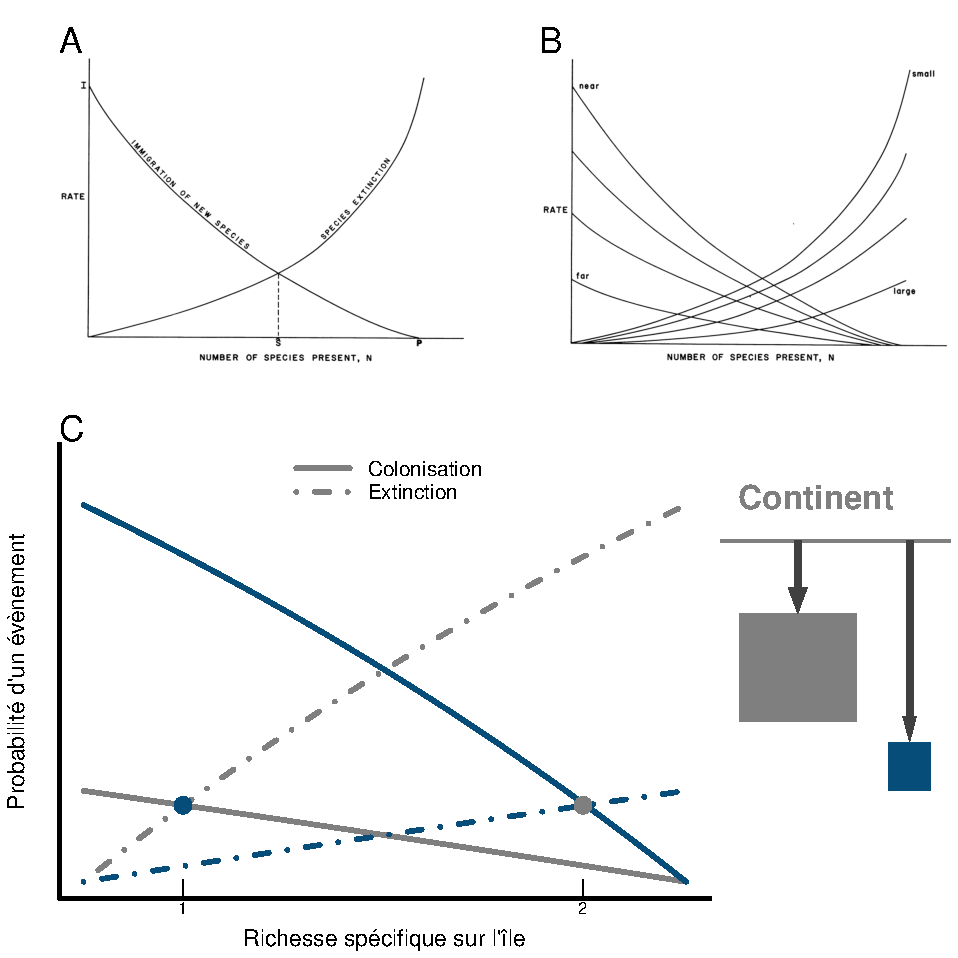
\includegraphics{fig/fig1.pdf}
\caption{\textbf{La Théorie de la biogéographie des Iles.} L'évolution
des taux de colonisation et d'extinction est présentée pour deux îles
aux caractéristiques différentes. Les tailles relatives des îles et les
distances qui les séparent du continent sont schématisées à droite du
graphique, les couleurs associent les îles à leurs courbes respectives.
Le pool d'espèce régional (\(P\)) est constitué de 100 espèces, les taux
de colonisation et d'extinction sont exprimés en terme de probabilité
d'évènement. Les points où colonisation et extinction s'équilibrent sont
marqué par les symboles en gris.\label{fig:figMW}}
\end{figure}

\subsection*{L'empreinte historique de la Théorie de la Biogéographie
des Iles de MacArthur et
Wilson}\label{lempreinte-historique-de-la-thuxe9orie-de-la-bioguxe9ographie-des-iles-de-macarthur-et-wilson}
\addcontentsline{toc}{subsection}{L'empreinte historique de la Théorie
de la Biogéographie des Iles de MacArthur et Wilson}

Dans leur livre \emph{The Theory of Island Biogeography}, MacArthur et
Wilson indique dans leur préface qu'il ne pensait pas que leur
résisterait longtemps surtout quand elle serait testé empiriquement :

\begin{quote}
We do not seriously believe that that the particular formulations
advanced in in the chapters to follow will fit for very long the
exacting results of future empirical invesitgation. (péface de l'édition
de 1967)
\end{quote}

Et pourtant fort près de 50 ans après la parution de leur ouvrage, la
vision distilé est toujours aussi vive en témoigne le livre paru en 2010
\emph{The Theory of Island Biogeography Revisited} (Losos and Ricklefs,
2010) et la reve par Warren et collègue (Warren et al., 2015) qui montre
bien que les île ont servie de moèdeles et que la vision est un point
les travaux sont capitale.

Le terme des îles est centraled mais il s'agit bien d'une théorie de la
biogéogroahie. reflète aussi l'importance des îles dans l'édification
d'une théorie isolation lux de migraotion simple / assemblage moins
nombreux / conséquence d'une manipultion limité à l'île / 5\% mais
répétable ? / un oacth isolé et peut être que flux au île (Simberloff,
1974) Pourquoi les îles en fait isolé flux et gros contraste mailand -
island alors qu'elles sontproches.. Les îles qui occupent le coeur de
l'ouvrage de Wallace et de MAcArthur et Wilson ont été essentiel poour
comprendre les processus qui forme la sitributn des espèces. Elle sosn
tproches du continent et peuvent être si différenetes la nature eotique
des piles à forcer les auteurs à comprendre l'origine de leur
singularit.é et ces sur ces bout de terre isolé qu'ils ont trouv.s des
réposnes historques ais ausso spataile qui a parmis d'aller vers des
dévelppemnt encore aujourd'hui très actis. La quête de cees honmes et de
bien d'autres reste finalemnt de comprendre pourquoi les espèces sont ou
elles sont et de comproendre ce qui les amanerner la. Meilleur
explication pour des arrangemnets spatiaux singuliers sont des processus
temporels. Faire émerger des règles mon apport amener des interactions.

Preston 1962 a lié species abundance et =\textgreater{} impact enorme
sur la conservation et encore aujourd'hui bien que simplifié les calculs
permettent de comprendredsimplementr dans quelles directions nous allons
{[}article NewYork Times{]} Malgré la 50 ans de depuis la publication du
Livre et premier articles a lasuorise de auiteure eux meme
=\textgreater{} publications récentes qui repartent de la théorie des
îles ; l'ecolet Warren et gravel and all

Dans la réédition de 2001 {[}{]} Wilson rappelle que le problème :

\begin{quote}
``The flaws of the book lie in its oversimplification and
incompleteness, which are endemic to most efforts at theory and
synthesis.''
\end{quote}

Diminuer la composante historqiue à la recherche de loi et j'ajouterais
aussi simple soit elle raffiner par la suite

\subsubsection{théorie de la niche}\label{thuxe9orie-de-la-niche}

\subsubsection{La théorie des
métapopulations}\label{la-thuxe9orie-des-muxe9tapopulations}

=\textgreater{} chapitre de Hanski

\subsubsection{La théorie neutre de l'écologie et le débat qu'elle
soulève}\label{la-thuxe9orie-neutre-de-luxe9cologie-et-le-duxe9bat-quelle-souluxe8ve}

Ecological equivalence des individus OK mais peut-être que l'abondance
des interactions expliques aussi

=\textgreater{} chapitre dans revisited

Problème si explication alternatives possibles alors on n'est pas obligé
de mettre pour expliquer quoi que ce soit. De plus savons nous si c'est
discernable ??? Si le deux relation aire espèce sont différentes d'un
groupe à l'autre alors oui\ldots{} Mais sinon\ldots{} Non.

Oppositon à la niche.

(Chapitre 8 TIB first paragraph)

Le concept récent de biodiversité. However ecological equivalence in
``the niche is a mapping of population dynamics onto this space''
({\textbf{???}}) vers le fonctionnemt des ecosystèmes levier d'action
vers une approche plus utilitariste mais qui donne uns certaine
proximité avec les eécosytèmes Loreau et al. (2001)

\subsection{Aller plus loin, Enjeux
théoriques}\label{aller-plus-loin-enjeux-thuxe9oriques}

L'effort théorique nécessaire en biogéographie porte sur l'intégration
ordonnée de concepts clés issus de différents champs de l'écologie
\cite{Thuiller2013}. Ainsi, alors que les conditions climatiques et plus
généralement la géographie physique sont classiquement évoquées pour
expliquer la répartition des espèces \cite{Kearney2004}, les
interactions entre espèces sont quant à elles souvent occultées. De
même, bien que les processus évolutifs soient souvent évoqués comme
déterminants majeurs de la diversité des espèces \cite{Rosindell2011},
leurs effets à court terme sont souvent ignorés \cite{Parmesan2006} dans
les scénarios décrivant la biodiversité de demain \cite{Lavergne2010}.
La difficulté principale est alors de produire des modèles (théoriques
en première instance) qui intègrent l'ensemble des processus et les
relations qu'ils entretient \cite{Thuiller2013} tout en gardant une
relative simplicité. Une théorie intégrative en biogéographie pourrait
être le meilleur point d'ancrage pour construire de nouvelles approches
appliquées. Avec une telle théorie en main, nous pourrions aller vers
l'enjeux majeurs de ces dernières années en biogéographie : relâcher les
hypothèses que les modèles classiques de répartitions des espèces
d'aujourd'hui utilisent (notamment en occultant les interactions) pour
prédire la biodiversité de demain \cite{Guisan2011}.

Dans le projet ici présenté, nous proposons de construire des modèles
théoriques plus intégratifs en repartant d'un modèle théorique
classique, celui de la théorie de la biogéographie des îles proposée par
MacArthur et Wilson \cite{MacArthur1967}. Dans un premier temps, nous y
ajoutons les interactions entre espèces et une relation explicite avec
l'environnement abiotique au travers d'une approche communauté centrée
qui étend le modèle classique. Dans un second temps, nous combinons une
approche population centrée et les processus évolutifs pour une
biogéographie insulaire plus mécaniste. Enfin, au regard des enjeux que
soulève le rôle des interactions entre espèces dans la construction de
la biodiversité, nous réfléchissons sur l'inférence d'espèces
interdépendantes.

différentes théories pour différentes échelles ??

De part son pouvoir explicatif et son élégance, le modèle de MacArthur
et Wilson est un point de départ approprié pour construire des modèles
plus intégratifs en intégrant explicitement des processus écologiques et
évolutifs. Cette idée n'est pas nouvelle et les auteurs de la TIB ont
étudié un certain nombre de processus écologiques. Notamment, ils ont
intégré les phénomènes de spéciation \cite{MacArthur1967} et réfléchis
sur l'importance des interactions quant à la répartition des espèces
\cite{MacArthur1984}. Néanmoins, dans le modèle classique, l'ensemble de
ces aspects sont absents, l'idée que les processus écologiques importent
peu aux larges échelles domine. Nous allons, dans ce projet, à
l'encontre de cette idée et proposons de construire des modèles
intégratifs qui étendent la TIB.

isolation / faune particulière des îles

\section*{Le rôle des interactions dans la distribution des
espèces}\label{le-ruxf4le-des-interactions-dans-la-distribution-des-espuxe8ces}
\addcontentsline{toc}{section}{Le rôle des interactions dans la
distribution des espèces}

L'objet central de ma thèse est l'introduction de ma thèse est d'essayer
de regrader la théorie de la biogéographie et notamment quelles
onfornatiosn 'écologie des réseayx peurt ameenr de la lumière sur la
théorie. Dans cette dernière partie de mon introduction, je présente
avec pkus de délément l'importance de l'intriduction des onteractions
dans une théorie de la biogéographie. Cela me permettra d'introduire nes
contributions qui seront détaillées dans ma thèse.

Wallace conclut :28 qu'une théorie générale doit tenir compte des
variation range et proximité des espèces porches et des overlapp.

\begin{quote}
Both competition and predation appear now to be much more important in
biogeography than people had formely guesses
\end{quote}

\subsection{Pourquoi les intéractions ne joue-t-elle pas un rôle
majeur}\label{pourquoi-les-intuxe9ractions-ne-joue-t-elle-pas-un-ruxf4le-majeur}

\subsubsection{La théorie de la biogéograohie ne les nient pas bien au
contraire}\label{la-thuxe9orie-de-la-bioguxe9ograohie-ne-les-nient-pas-bien-au-contraire}

La théorie de la Biogéographie des îles (et il en va de même pour la
théorie neutre) est certes une théorie qui ne s'articule pas sur les
interactions et fais une forme d'équivalence écologique, les idées sont
clairemnent oser que localemnt les raisons profindes de l'extinciton
locale. La question que l'on peut alors se poser est de savoir si les
c'est si on peut aller plus loin qu'une simple enonciation des proncipes
tout en gardante une cohérence. Aiinsi i lsemble omportant que la
théorie de la Biog.éogrpahie doit intégrer des résultats précis en terme
de réseaux. Dans le premier chapitre j'ai poursuivi cette idées et est
montré qu'une approche communait centrés pouvat être prpoposé. Ne pas
considéere mdes espèces mais des aassembalges est une bonne échelle pour
aborder des problèmes des conséquences écologques des transients. Il est
aussi int.ressant que cela nous a fait glissé vers la compréhension des
résulats qu'om doit avoir dans les données de co-occurrene.

Accent sur les cascading effect est surtout un problème de l'instabiilté
({\textbf{???}}) Il ya aussi l'article perturbant de Säterberg et al.
(2013) qui montre que le fait qu'une espèce soit (ex. pêche) peut
conduirte à des extinctions d'autres espèces lié dans le réseau\ldots{}
Ces deux exemple montrent que les interactions peuvent mener à des
problèmes de prédicitons et donc porblèmes sur prévoir les services
ecosystémiques et c'est appuyer par Cahill et al. (2013) qui nous
indique en somme que le changemment des interactiosn biotiques ets la
voie privilégiée d'extintionciton dans un contexte de changement
climatique.

chap 2 geographical ecology

il prend comme exemple la compétition entre oiseau et un manque de
ressource pour une année partiuculièremnet sévère et que 19 and pas
assez pour voir et il conclut que

\begin{quote}
This is the main reason most evidence for competition is from
biogepgraphers.
\end{quote}

Distributiin des fauvettes \emph{Crateroscelis robusta} et \emph{C.runa}

Mais le p

\subsubsection{Problème d'échelle}\label{probluxe8me-duxe9chelle}

Oubli de ce facteur important de Ls SMDS\ldots{}

Les interactions intra et inter spécifiques constituent un facteur
rapidement pressenti comme responsable de la distribution spatiale des
espèces \cite{Levin1974}. L'interdépendance des espèces conditionne, en
effet, l'aspect favorable de l'environnement au sens large (biotique et
abiotique). Ainsi Godsoe \textit{et al.} 2012, mettent en équations le
caractère favorable de l'environnement pour une espèce donnée en terme
de probabilité de présence d'une autre espèce et de la nature de leur
interaction \cite{Godsoe2012}. De même, Holt et Barfield 2009 montrent
l'impact de la prédation sur la répartition d'espèces en compétition
\cite{Holt2009} insistant ainsi sur le rôle majeur des interactions.
Davis \textit{et al.} 1998 ont montrés que, pour trois drosophiles en
compétition, l'effet d'un parasitoïde n'est pas le même le long d'un
gradient selon que les espèces sont seules ou ensemble \cite{Davis1998}.
Récemment, des efforts ont été réalisés pour mettre en évidence
l'importance de l'interdépendance des espèces dans les données aux
larges échelles spatiales \cite{Gotelli2010}. On trouve actuellement
dans la littérature une grande motivation pour les intégrer dans les
modèles de distribution d'espèces \cite{Kissling2011, Guisan2011}. Des
efforts théoriques sont encore nécessaires pour arriver à de telles
approches. Néanmoins, rapprocher différents champs de l'écologie peut
s'avérer d'une utilité majeure. Jabot et Bascompte \cite{Jabot2012}
2012, ont d'ailleurs montré l'importance des interactions pour
comprendre la distribution des espèces en rapprochant écologie des
réseaux et un modèle de metacommunauté. De même Gravel \textit{et al.}
2011 \cite{Gravel2011b} introduise l'interdépendance proie-prédateur
dans le modèle classique de MacArthur et Wilson menant aux prémices
d'une théorie trophique de la biogéographie des îles.

L'ajout des interactions dans un modèle incluant l'environnement
abiotique interroge la relation que les deux processus entretiennent. Si
les espèces n'ont pas les mêmes performances dans différents milieux du
fait de leur physiologie, pour les mêmes espèces considérées, les
réseaux n'ont pas de raison d'être identiques d'un milieu à un autre.
C'est sur ce fait que Poisot \textit{et al.} 2012 ont proposé une mesure
de dissimilarité des réseaux \cite{Poisot2012}. Defossez \textit{et al.}
montrent que les interactions négatives entre l'hêtre commun
(\textit{Fagus Sylvaitca}) et les micro-organismes du sol diminuent avec
l'altitude \cite{Defossez2011}. Ainsi, les contraintes biotiques sont à
relier à l'environnement \cite{Brooker2006,Canham2006} et un modèle
intégratif doit donner un cadre cohérent à ces rétroactions entre
processus. Enfin, l'importance des interactions est à mettre en relation
avec l'échelle considérée \cite{Peterson2011}. Pour deux espèces en
interaction, plus l'échelle d'étude est large, moins les effets des
interactions locales sont susceptibles d'être capturés, le pouvoir
explicatif de la présence d'une espèce sur l'autre peut être alors
discutable \cite{Araujo2007}. Comprendre quels sont les processus à
prendre en compte aux différentes échelles spatio-temporelles et
comprendre comment le changement d'échelle affecte nous prédictions est
aussi un véritable challenge en biogéographie \cite{Martinez2012}.

\subsubsection{Un problème d'échelle
?}\label{un-probluxe8me-duxe9chelle}

Comment les varitions démogrpahiques interactions se propagent-t-elle à
travers les échelles spatiale.

\begin{quote}
However, it is argued that applying bio-climatic models at macro-scales,
where climatic influences on species distributions are shown to be
dominant, can minimize the impact of biotic interactions. Indeed, the
fact that a number of bioclimatic models have been highly successful at
simulating current species distributions at certain scales is in
fundamental disagreement with the proposition that species distributions
cannot be adequately defined by climatic factors alone. (Pearson and
Dawson, 2003)
\end{quote}

\begin{quote}
We will never be able to predict the future with accuracy, but we need a
strategy for using existing knowledge and bioclimatic modeling to
improve understanding of the likely effects of future climate on
biodiversity. (Araujo and Rahbek, 2006).
\end{quote}

Les ranges comme un fait (wallace chap 2) des espèces avec des larges
avec des grandes ranges Loddigésie admirable (\emph{Loddigesia
mirabilis}) seul collibris de son genre vs Lièvre variable (\emph{Lepus
timidus}) nomnbre d'espèce dans un genre vaire beaucoup =\textgreater{}
un autre indice de solution pas fructifiées\ldots{} Pithacia Monathus vs
Pithecia pythecia separé par une rivière Geographical Ecology
=\textgreater{} patterns in the distribution of spceies 2 espèces
proches des ranges très séparéed =\textgreater{} species Bonobo et
cChimpanzés

orblème étant que le signal n'est visible que si on a des données sur
20and.

Le problème

Parallèle entre information des traits sur le régime allimentaire et
l'information dans les ranegs est-ce cela qui conduit les ecologistes à
être des statisticuencs. et l'info dans l'ADN

\subsection{Faire un questionnement des intersections des ranges et des
règles}\label{faire-un-questionnement-des-intersections-des-ranges-et-des-ruxe8gles}

On a besoinde rule on reste descriptive il y a des relation
EH-Bioversité, SAR, Diversité-équilibre diversité fonctionnenemnt qui
sont partielelemnt reliées et des théries débat theories neutre theéor
de la niche Stein et al. (2014). Dans cette review Stein et al. (2014)
montre que vegetaiton est inportnates ce qui eimplique des
inbteractions. Théorie allométrique prometteuse en ce sens qu'elle loi
physiques. Différents concept autrour d'une même notion sur plusieurs
paradigme pour une même notion sur les metacommunity Leibold et al.
(2004) il peuvent co-exister mais faudrait les savoir ce qui fait qu'on
a pus l'un ou l'autr.

La puissance de la Biogéographie est aussi sont implications dans des
cas très concrets Cirtwill and Stouffer (2015) mais aussi ne puissance
exploratoire théoriques Gravel et al. (2011) Cazelles et al. (2015) des
îles l'idée des interactions à déjà montré ça pertinence sur plusieurs
exemples. Cirtwill and Stouffer (2015)

Les interactions quelles pourrait être leur conséquence à large échelle
?

\begin{quote}
(:154) ``Does the environment dictate the structure of the community, or
are the species a fairly random assemblage?
\end{quote}

Cette id.e aussi est données par

\begin{quote}
A few decades ago it as fashionable for ecologist to study communities
in the arctic on the grounds that these would be very simple communities
and hence easy to understand. Many excellent ecologists still follow
this belied, but there are others who feel that it may be easier to
understand the extremely complex communities. This sounds paradoxical:
How can a more complex communities by easier to understand? A possible
answer might be that complex community has has strong interactions among
species so that the lives of the separate species are less independent
than in a simple community. Where there is greater interdependence,
patterns may be more conspicuous."
\end{quote}

Information dans les distributions gecko australien généraliste
\emph{Heteronotia binoei} =\textgreater{}~alors peut être que ça marche
bien mais sur une espèce spécialiste ??

\begin{quote}
Generalist consumers should typically be weakly coupled to any one of
their prey populations because, when feeding on many different species,
they cannot be strongly coupled to any one of them Murdoch et al. (2002)
\end{quote}

Intégrations des contraintes biotiques et de la théorie à la recherche
de signaux de d'intéraction

Dans ma thèse j'ai oassé du temps à essayer de mettre au point un modèke
qui donnait de la substace aux idées de MacArthur et Wilson een etandant
le travai initié par Gravel et collègues pour aller plus loin dans la
compréhension des effets joints des interactions et des contraintes
abiotiques. C'est aussi ce qui m'a animé pour en mettre en place la
compréhesin dans les données de co-occurrence avant d'aller m'y
confronter frongalemnet. Ma dernière intergtaion a Été de trouver des
pistes pour allerr plus loin dans la théorie et explorer des pistes que
je n'avais pas encore dxplorer mais qui seront à court terme les
directions que je souhaite explorer.

Abondance des données Les atouts actuels de la biogéographie sont 1- une
quantité importante d'information relative aux présences d'espèces et au
climat et 2- des modèles corrélatifs puissants qui décrivent précisément
le lien entre l'espèce et son environnement abiotique. Le terme
abiotique peut prêter à confusion dans la mesure où les espèces
elles-mêmes peuvent modifier des variables dîtes abiotiques. Par
exemple, les végétaux peuvent avoir un grand impact sur les variables
abiotiques locales comme la température et l'humidité du sol
\cite{Breshears1998}. Certains auteurs font une distinction précise en
utilisant les termes de \textit{scenopoetiques} pour les variables
environnementales sur lesquels les espèces ne peuvent influer et de
\textit{dynamiquement liées} pour les autres \cite{Peterson2011}. Nous
occulterons volontairement ces-dernières, l'environnement abiotique dont
il est ici question n'est donc pas dynamiquement lié aux espèces.

Partir du development de la niche et des hypotheses clef comme
l'heterogeneité spatiale qui peut accroitre la biodiversité un exemple
c'est les ecoulemnents à petites faible echelles de l'hydrologie niche
hdrologique à fable échelles Letten et al. (2015) repartition
hydrologique les hypothèses sont qui explique celon les différentes
besoin des espèces (principes de la niche) que besoin différemtes me
répartition des espèces. Cette idées est

Mais une espèce généraliste autant que sécialiste Poisot et al. (2015)

A large espes répartition de la biodiversité on quantifie la différence
depuis les mesures classiques. Simpson, alpha gamma beta qui sont
étendues au réseau Poisot et al. (2012). Mais quand on chnage d'echelle
on arrive rarement à quelques choses de concluant pour l'integration des
interactions. Pourtant il ya des exemples convaicant comme celui de
Gitelli.

-- conclure en repartant sur l'exemple détaillé. Vespa aussi au Amérqieu
la densit. des traffic\ldots{} Multi couche de distrobution dans le cas
du frelon asiatique Villemant et al. ({\textbf{???}}) ont montrés que
superposition du genre \emph{Vespa} et notamment au niveau asiatique
énormément aisin l'inférence se fait sur des données qui comporte une
empreinte de condition et localemnt éteinte alors que possiblement
comtraite qui ne seront pas en France\ldots{} Essyer de faire des cartes
de risques plutôt que de constater après coup\ldots{} Après avoir fait
un retour sur plus de biologie je m,intergoge sur lesquelle dans la
suiste Dépasser les questionnemnet sur les espèces la contrainte il me
semble qu'une piste c'est aouverte avec des questions énergétique on se
rencontre qu'il y a des base én.ergétiqe dcommunet et que c'est ancrage
sit beaoup\ldots{}

\subsection{Au dela desinteractioms}\label{au-dela-desinteractioms}

La bonne unité d'analyse ? D'où parti r? la question a été pourquoi il y
a autant d'espèces mais je pense qu'un equestion légèremnetn différentes
n'a pas été assez invextie : pourquoi peuvent-elles être si
nombreuse\ldots{}. La limite est toujours OK si assez pour 2 ou plus. Et
pourquoi pas une pourquoi pas une espèce de taille ++

\hypertarget{refs}{}
\hypertarget{ref-Allesina2012a}{}
Allesina, S., Tang, S., 2012. Stability criteria for complex ecosystems.
Nature 483, 205--208.
doi:\href{https://doi.org/10.1038/nature10832}{10.1038/nature10832}

\hypertarget{ref-TheArabidopsisGenomeInitiative2000}{}
Arabidopsis Genome Initiative, 2000. Analysis of the genome sequence of
the flowering plant Arabidopsis thaliana. Nature 408, 796--815.
doi:\href{https://doi.org/10.1038/35048692}{10.1038/35048692}

\hypertarget{ref-Araujo2006}{}
Araujo, M.B., Rahbek, C., 2006. How Does Climate Change Affect
Biodiversity? Science 313, 1396--1397.
doi:\href{https://doi.org/10.1126/science.1131758}{10.1126/science.1131758}

\hypertarget{ref-Beck2012}{}
Beck, J., Ballesteros-Mejia, L., Buchmann, C.M., Dengler, J., Fritz,
S.A., Gruber, B., Hof, C., Jansen, F., Knapp, S., Kreft, H., Schneider,
A.-K., Winter, M., Dormann, C.F., 2012. What's on the horizon for
macroecology? Ecography 35, 001--011.
doi:\href{https://doi.org/10.1111/j.1600-0587.2012.07364.x}{10.1111/j.1600-0587.2012.07364.x}

\hypertarget{ref-Beck2014a}{}
Beck, J., Böller, M., Erhardt, A., Schwanghart, W., 2014. Spatial bias
in the GBIF database and its effect on modeling species' geographic
distributions. Ecological Informatics 19, 10--15.
doi:\href{https://doi.org/10.1016/j.ecoinf.2013.11.002}{10.1016/j.ecoinf.2013.11.002}

\hypertarget{ref-Bellard2012}{}
Bellard, C., Bertelsmeier, C., Leadley, P., Thuiller, W., Courchamp, F.,
2012. Impacts of climate change on the future of biodiversity. Ecology
letters 15, 365--377.
doi:\href{https://doi.org/10.1111/j.1461-0248.2011.01736.x}{10.1111/j.1461-0248.2011.01736.x}

\hypertarget{ref-Cahill2013}{}
Cahill, A.E., Aiello-Lammens, M.E., Fisher-Reid, M.C., Hua, X.,
Karanewsky, C.J., Ryu, H.Y., Sbeglia, G.C., Spagnolo, F., Waldron, J.B.,
Warsi, O., Wiens, J.J., 2013. How does climate change cause extinction?
Proceedings. Biological sciences / The Royal Society 280, 20121890.
doi:\href{https://doi.org/10.1098/rspb.2012.1890}{10.1098/rspb.2012.1890}

\hypertarget{ref-Cazelles2015b}{}
Cazelles, K., Mouquet, N., Mouillot, D., Gravel, D., 2015. On the
integration of biotic interaction and environmental constraints at the
biogeographical scale. Ecography n/a--n/a.
doi:\href{https://doi.org/10.1111/ecog.01714}{10.1111/ecog.01714}

\hypertarget{ref-Cirtwill2015}{}
Cirtwill, A.R., Stouffer, D.B., 2015. Knowledge of predator-prey
interactions improves predictions of immigration and extinction in
island biogeography. Global Ecology and Biogeography n/a--n/a.
doi:\href{https://doi.org/10.1111/geb.12332}{10.1111/geb.12332}

\hypertarget{ref-Connor1979}{}
Connor, E.F., Simberloff, D., 1979. The Assembly of Species Communities:
Chance or Competition? Ecology 60, 1132.
doi:\href{https://doi.org/10.2307/1936961}{10.2307/1936961}

\hypertarget{ref-Diamond1975}{}
Diamond, J.M., 1975. Assembly of species communities, in: Cody, M.L.,
Diamond, J.M. (Eds.), Ecology and Evolution of Communities. Harvard
University Press, Cambridge, Massachusetts, USA., pp. 342--444.

\hypertarget{ref-Elith2006}{}
Elith, J., H. Graham, C., P. Anderson, R., Dudík, M., Ferrier, S.,
Guisan, A., J. Hijmans, R., Huettmann, F., R. Leathwick, J., Lehmann,
A., Li, J., G. Lohmann, L., A. Loiselle, B., Manion, G., Moritz, C.,
Nakamura, M., Nakazawa, Y., McC. M. Overton, J., Townsend Peterson, A.,
J. Phillips, S., Richardson, K., Scachetti-Pereira, R., E. Schapire, R.,
Soberón, J., Williams, S., S. Wisz, M., E. Zimmermann, N., 2006. Novel
methods improve prediction of species' distributions from occurrence
data. Ecography 29, 129--151.
doi:\href{https://doi.org/10.1111/j.2006.0906-7590.04596.x}{10.1111/j.2006.0906-7590.04596.x}

\hypertarget{ref-Elith2009a}{}
Elith, J., Leathwick, J.R., 2009. Species Distribution Models:
Ecological Explanation and Prediction Across Space and Time. Annual
Review of Ecology, Evolution, and Systematics 40, 677--697.
doi:\href{https://doi.org/10.1146/annurev.ecolsys.110308.120159}{10.1146/annurev.ecolsys.110308.120159}

\hypertarget{ref-Engelbrecht2007}{}
Engelbrecht, B.M.J., Comita, L.S., Condit, R., Kursar, T. a, Tyree,
M.T., Turner, B.L., Hubbell, S.P., 2007. Drought sensitivity shapes
species distribution patterns in tropical forests. Nature 447, 80--82.
doi:\href{https://doi.org/10.1038/nature05747}{10.1038/nature05747}

\hypertarget{ref-Finstermeier2013}{}
Finstermeier, K., Zinner, D., Brameier, M., Meyer, M., Kreuz, E.,
Hofreiter, M., Roos, C., 2013. A Mitogenomic Phylogeny of Living
Primates. PLoS ONE 8, 1--10.
doi:\href{https://doi.org/10.1371/journal.pone.0069504}{10.1371/journal.pone.0069504}

\hypertarget{ref-Gravel2011c}{}
Gravel, D., Bell, T., Barbera, C., Bouvier, T., Pommier, T., Venail, P.,
Mouquet, N., 2011. Experimental niche evolution alters the strength of
the diversity--productivity relationship. Nature 469, 89--92.
doi:\href{https://doi.org/10.1038/nature09592}{10.1038/nature09592}

\hypertarget{ref-Hannah2013}{}
Hannah, L., Roehrdanz, P.R., Ikegami, M., Shepard, A.V., Shaw, M.R.,
Tabor, G., Zhi, L., Marquet, P.a., Hijmans, R.J., 2013. Climate change,
wine, and conservation. Proceedings of the National Academy of Sciences
110, 6907--6912.
doi:\href{https://doi.org/10.1073/pnas.1210127110}{10.1073/pnas.1210127110}

\hypertarget{ref-Hijmans2005}{}
Hijmans, R.J., Cameron, S.E., Parra, J.L., Jones, P.G., Jarvis, A.,
2005. Very high resolution interpolated climate surfaces for global land
areas. International Journal of Climatology 25, 1965--1978.
doi:\href{https://doi.org/10.1002/joc.1276}{10.1002/joc.1276}

\hypertarget{ref-Hortal2011}{}
Hortal, J., Diniz-Filho, J.A.F., Bini, L.M., Rodríguez, M.Á., Baselga,
A., Nogués-Bravo, D., Rangel, T.F., Hawkins, B.A., Lobo, J.M., 2011. Ice
age climate, evolutionary constraints and diversity patterns of European
dung beetles. Ecology Letters 14, 741--748.
doi:\href{https://doi.org/10.1111/j.1461-0248.2011.01634.x}{10.1111/j.1461-0248.2011.01634.x}

\hypertarget{ref-Kearney2004}{}
Kearney, M., Porter, W.P., 2004. MAPPING THE FUNDAMENTAL NICHE:
PHYSIOLOGY, CLIMATE, AND THE DISTRIBUTION OF A NOCTURNAL LIZARD. Ecology
85, 3119--3131.
doi:\href{https://doi.org/10.1890/03-0820}{10.1890/03-0820}

\hypertarget{ref-Kefi2015}{}
Kéfi, S., Berlow, E.L., Wieters, E.A., Joppa, L.N., Wood, S.A., Brose,
U., Navarrete, S.A., 2015. Network structure beyond food webs: mapping
non-trophic and trophic interactions on Chilean rocky shores. Ecology
96, 291--303.
doi:\href{https://doi.org/10.1890/13-1424.1}{10.1890/13-1424.1}

\hypertarget{ref-Kefi2012}{}
Kéfi, S., Berlow, E.L., Wieters, E.A., Navarrete, S.A., Petchey, O.L.,
Wood, S.A., Boit, A., Joppa, L.N., Lafferty, K.D., Williams, R.J.,
Martinez, N.D., Menge, B.A., Blanchette, C.A., Iles, A.C., Brose, U.,
2012. More than a meal\ldots{} integrating non-feeding interactions into
food webs. Ecology Letters 15, 291--300.
doi:\href{https://doi.org/10.1111/j.1461-0248.2011.01732.x}{10.1111/j.1461-0248.2011.01732.x}

\hypertarget{ref-Koh2004}{}
Koh, L.P., 2004. Species Coextinctions and the Biodiversity Crisis.
Science 305, 1632--1634.
doi:\href{https://doi.org/10.1126/science.1101101}{10.1126/science.1101101}

\hypertarget{ref-Leibold2004}{}
Leibold, M.a., Holyoak, M., Mouquet, N., Amarasekare, P., Chase, J.M.,
Hoopes, M.F., Holt, R.D., Shurin, J.B., Law, R., Tilman, D., Loreau, M.,
Gonzalez, a., 2004. The metacommunity concept: a framework for
multi-scale community ecology. Ecology Letters 7, 601--613.
doi:\href{https://doi.org/10.1111/j.1461-0248.2004.00608.x}{10.1111/j.1461-0248.2004.00608.x}

\hypertarget{ref-Letten2015}{}
Letten, A.D., Keith, D.a., Tozer, M.G., Hui, F.K., 2015. Fine-scale
hydrological niche differentiation through the lens of multi-species
co-occurrence models. Journal of Ecology 103, 1264--1275.
doi:\href{https://doi.org/10.1111/1365-2745.12428}{10.1111/1365-2745.12428}

\hypertarget{ref-Lomolino2000}{}
Lomolino, M.V., 2000. A call for a new paradigm of island biogeography.
Global Ecology and Biogeography 9, 1--6.
doi:\href{https://doi.org/10.1046/j.1365-2699.2000.00185.x}{10.1046/j.1365-2699.2000.00185.x}

\hypertarget{ref-Loreau2001}{}
Loreau, M., Naeem, S., Inchausti, P., Bengtsson, J., Grime, J.P.,
Hector, a, Hooper, D.U., Huston, M. a, Raffaelli, D., Schmid, B.,
Tilman, D., Wardle, D. a, 2001. Biodiversity and ecosystem functioning:
current knowledge and future challenges. Science (New York, N.Y.) 294,
804--8.
doi:\href{https://doi.org/10.1126/science.1064088}{10.1126/science.1064088}

\hypertarget{ref-Losos2010}{}
Losos, J.B., Ricklefs, R.E., 2010. The Theory of Island Biogeography
Revisited. Princeton University Press, Princeton, NJ.

\hypertarget{ref-macarthur1972geographical}{}
MacArthur, R.H., 1972. Geographical Ecology: Patterns in the
Distribution of Species, Biology / {[}princeton university press{]}.
Princeton University Press.

\hypertarget{ref-MacArthur1967}{}
MacArthur, R.H., Wilson, E.O., 1967. Theory of Island Biogeography,
Princeton landmarks in biology. Princeton University Press, Princeton,
NJ.

\hypertarget{ref-May2004}{}
May, R.M., 2004. Uses and abuses of mathematics in biology. Science (New
York, N.Y.) 303, 790--3.
doi:\href{https://doi.org/10.1126/science.1094442}{10.1126/science.1094442}

\hypertarget{ref-May1973}{}
May, R.M., 1973. Stability and complexity in model ecosystems.
Monographs in population biology 6, 1--235.
doi:\href{https://doi.org/10.1109/TSMC.1978.4309856}{10.1109/TSMC.1978.4309856}

\hypertarget{ref-mccann2011food}{}
McCann, K.S., 2011. Food Webs, Monographs in population biology.
Princeton University Press.

\hypertarget{ref-McCann2000}{}
McCann, K.S., 2000. The diversity-stability debate. Nature 405, 228--33.
doi:\href{https://doi.org/10.1038/35012234}{10.1038/35012234}

\hypertarget{ref-Montoya2009}{}
Montoya, J., Woodward, G., Emmerson, M.C., Solé, R.V., 2009. Press
perturbations and indirect effects in real food webs. Ecology 90,
2426--2433.
doi:\href{https://doi.org/10.1890/08-0657.1}{10.1890/08-0657.1}

\hypertarget{ref-Murdoch2002}{}
Murdoch, W.W., Kendall, B.E., Nisbet, R.M., Briggs, C.J., McCauley, E.,
Bolser, R., 2002. Single-species models for many-species food webs.
Nature 417, 541--543.
doi:\href{https://doi.org/10.1038/417541a}{10.1038/417541a}

\hypertarget{ref-Pascual2006}{}
Pascual, M., Dunne, J.A., 2006. Ecological Networks: Linking Structure
to Dynamics in Food Webs. Oxford University Press.

\hypertarget{ref-Pearson2003}{}
Pearson, R.G., Dawson, T.P., 2003. Predicting the impacts of climate
change on the distribution of species: are bioclimate envelope models
useful? Global Ecology and Biogeography 12, 361--371.
doi:\href{https://doi.org/10.1046/j.1466-822X.2003.00042.x}{10.1046/j.1466-822X.2003.00042.x}

\hypertarget{ref-Pelletier2007}{}
Pelletier, F., Clutton-Brock, T., Pemberton, J., Tuljapurkar, S.,
Coulson, T., 2007. The evolutionary demography of ecological change:
Linking trait variation and population growth. Science 315, 1571--1574.
doi:\href{https://doi.org/10.1126/science.1139024}{10.1126/science.1139024}

\hypertarget{ref-Poisot2012}{}
Poisot, T., Canard, E., Mouillot, D., Mouquet, N., Gravel, D., Jordan,
F., 2012. The dissimilarity of species interaction networks. Ecology
letters 15, 1353--61.
doi:\href{https://doi.org/10.1111/ele.12002}{10.1111/ele.12002}

\hypertarget{ref-Poisot2015c}{}
Poisot, T., Kéfi, S., Morand, S., Stanko, M., Marquet, P.A., Hochberg,
M.E., 2015. A continuum of specialists and generalists in empirical
communities. PLoS ONE 10, 1--12.
doi:\href{https://doi.org/10.1371/journal.pone.0114674}{10.1371/journal.pone.0114674}

\hypertarget{ref-Razafindratsima2013}{}
Razafindratsima, O.H., Mehtani, S., Dunham, A.E., 2013. Extinctions,
traits and phylogenetic community structure: Insights from primate
assemblages in Madagascar. Ecography 36, 047--056.
doi:\href{https://doi.org/10.1111/j.1600-0587.2011.07409.x}{10.1111/j.1600-0587.2011.07409.x}

\hypertarget{ref-Saterberg2013}{}
Säterberg, T., Sellman, S., Ebenman, B., 2013. High frequency of
functional extinctions in ecological networks. Nature 499, 468--70.
doi:\href{https://doi.org/10.1038/nature12277}{10.1038/nature12277}

\hypertarget{ref-Schoener2011a}{}
Schoener, T.W., 2011a. The Newest Synthesis : Understanding Ecological
Dynamics. Science 331, 426--429.
doi:\href{https://doi.org/10.1126/science.1193954}{10.1126/science.1193954}

\hypertarget{ref-Schoener2011}{}
Schoener, T.W., 2011b. The newest synthesis: understanding the interplay
of evolutionary and ecological dynamics. Science (New York, N.Y.) 331,
426--9.
doi:\href{https://doi.org/10.1126/science.1193954}{10.1126/science.1193954}

\hypertarget{ref-Simberloff1974a}{}
Simberloff, D.S., 1974. Equilibrium Theory of Island Biogeography and
Ecology. Annual Review of Ecology and Systematics 5, 161--182.
doi:\href{https://doi.org/10.1146/annurev.es.05.110174.001113}{10.1146/annurev.es.05.110174.001113}

\hypertarget{ref-Simberloff1969}{}
Simberloff, D.S., Wilson, E.O., 1969. Experimental Zoogeography of
Islands: The Colonization of Empty Islands. Ecology 50, 278--296.
doi:\href{https://doi.org/10.2307/1934856}{10.2307/1934856}

\hypertarget{ref-Springer2015}{}
Springer, A., Swann, D., Crimmins, M., 2015. Climate change impacts on
high elevation saguaro range expansion. Journal of Arid Environments
116, 57--62.
doi:\href{https://doi.org/10.1016/j.jaridenv.2015.02.004}{10.1016/j.jaridenv.2015.02.004}

\hypertarget{ref-Stein2014}{}
Stein, A., Gerstner, K., Kreft, H., 2014. Environmental heterogeneity as
a universal driver of species richness across taxa, biomes and spatial
scales. Ecology Letters n/a--n/a.
doi:\href{https://doi.org/10.1111/ele.12277}{10.1111/ele.12277}

\hypertarget{ref-Thuiller2013}{}
Thuiller, W., Münkemüller, T., Lavergne, S., Mouillot, D., Mouquet, N.,
Schiffers, K., Gravel, D., 2013. A road map for integrating
eco-evolutionary processes into biodiversity models. Ecology Letters 16,
94--105. doi:\href{https://doi.org/10.1111/ele.12104}{10.1111/ele.12104}

\hypertarget{ref-Vanbergen2013}{}
Vanbergen, A.J., 2013. Threats to an ecosystem service: Pressures on
pollinators. Frontiers in Ecology and the Environment 11, 251--259.
doi:\href{https://doi.org/10.1890/120126}{10.1890/120126}

\hypertarget{ref-Waldrop2016}{}
Waldrop, M.M., 2016. The hundred-year quest for gravitational waves ---
in pictures. Nature.
doi:\href{https://doi.org/10.1038/nature.2016.19340}{10.1038/nature.2016.19340}

\hypertarget{ref-wallace1881island}{}
Wallace, A.R., 1881. Island Life: Or, The Phenomena and Causes of
Insular Faunas and Floras, Including a Revision and Attempted Solution
of the Problem of Geological Climates. Harper \& brothers.

\hypertarget{ref-Wallace1860}{}
Wallace, A.R., 1860. On the Zoological Geography of the Malay
Archipelago. Journal of the Proceedings of the Linnean Society of
London. Zoology 4, 172--184.
doi:\href{https://doi.org/10.1111/j.1096-3642.1860.tb00090.x}{10.1111/j.1096-3642.1860.tb00090.x}

\hypertarget{ref-Wallace1858}{}
Wallace, A.R., 1858. On the Tendency of Varieties to depart indefinitely
from the Original Type. Proceedings of the Linnean Society Of London 3,
53--62.

\hypertarget{ref-Warren2015}{}
Warren, B.H., Simberloff, D., Ricklefs, R.E., Aguilée, R., Condamine,
F.L., Gravel, D., Morlon, H., Mouquet, N., Rosindell, J., Casquet, J.,
Conti, E., Cornuault, J., Fernández-Palacios, J.M., Hengl, T., Norder,
S.J., Rijsdijk, K.F., Sanmartín, I., Strasberg, D., Triantis, K.A.,
Valente, L.M., Whittaker, R.J., Gillespie, R.G., Emerson, B.C., Thébaud,
C., 2015. Islands as model systems in ecology and evolution: Prospects
fifty years after MacArthur-Wilson. Ecology Letters 18, 200--217.
doi:\href{https://doi.org/10.1111/ele.12398}{10.1111/ele.12398}

\hypertarget{ref-Wootton1994a}{}
Wootton, J.T., 1994. The Nature and Consequences of Indirect Effects in
Ecological Communities. Annual Review of Ecology and Systematics 25,
443--466.
doi:\href{https://doi.org/10.1146/annurev.es.25.110194.002303}{10.1146/annurev.es.25.110194.002303}
